\cleardoublepage\documentclass[../main.tex]{subfiles}
\begin{document}
\chapter{Integral Definida}\label{cap:IntDef}\index{Integral!definida}
\minitoc
%\tableofcontents
\subsection*{Objetivos de aprendizagem do capítulo}
\addcontentsline{toc}{section}{Objetivos de aprendizagem do capítulo}
Ao final deste capítulo você deverá ser capaz de:
\begin{itemize}
    \item Conhecer o significado geométrico da integral definida;
    \item Identificar a existência das funções integráveis;
    \item Aplicar as propriedades de integral definida nos seus cálculos;
    \item Interpretar os teoremas fundamentais do cálculo integral;
    \item Interpretar corretamente a integral definida na aplicação do cálculo de áreas de regiões planas.
\end{itemize}

\section{Introdução}
A integral definida é um dos pilares do cálculo; é também uma ferramenta essencial para determinar quantidades importantes para a matemática, tais como áreas, volumes, comprimentos de curvas, entre outros. A ideia por trás da integral definida é independente a da integral indefinida, ou seja, não é como a operação inversa da derivada. Assim, poderemos calcular efetivamente as quantidades requeridas, dividindo-as em pequenas partes e, em seguida, somando-as para obter uma aproximação do valor desejado, que no limite torna-se exatamente o valor desejado.

Historicamente, as noções da integral definida remontam à Antiguidade, mas o conceito foi estabelecido apenas na era moderna como consequência da contribuição de muitos matemáticos tais como Newton e Leibniz, porém, foi o matemático Riemann, no século XIX, quem formulou o conceito utilizado atualmente.

Neste capítulo, trataremos da integral definida e estudaremos suas principais propriedades, dentre as quais ressaltamos os teoremas fundamentais do cálculo, que se relacionam com os conceitos da antiderivada de integral indefinida e da integral definida; estudaremos ainda as integrais impróprias úteis no tratamento de intervalos ilimitados; e por fim, apresentaremos algumas aplicações da integral definida no cálculo de áreas, volumes e comprimento de uma curva.

\section{Noção de integral}\label{cap_int_sec_nocaoint}

\subsection{Soma de Riemann}\index{Integral!soma de Riemann}\label{subsec:SomaRiemann}

Seja $f$ uma função contínua definida em um intervalo fechado $[a, b]$. Seja, também, $P$ a seguinte \emph{partição} de $[a, b]$
\begin{equation}
  P = \{a=x_0<x_1<x_2<\cdots<x_n=b\},
\end{equation}
onde $n+1$ é o número de pontos na partição. Definimos
\begin{equation}
  \Delta x_i = x_{i} - x_{i-1}
\end{equation}
o tamanho de cada subintervalo $I_{i} = [x_{i-1}, x_{i}]$ da partição, com $i = 1, 2, \cdots, n$. A \emph{norma da partição} é definida por
\begin{equation}
  \|P\| = \max_{i=1, \dotsc, n} \Delta x_i,
\end{equation}
 
i.e. o tamanho do maior subintervalo da partição. Com isso, chama-se de uma \emph{soma de Riemann} toda a expressão da forma
\begin{equation}
  S_n = \sum_{i=1}^n f(x_i^*)\Delta x_i,
\end{equation}
onde $x_i^*\in [x_i, x_{i-1}]$ (arbitrariamente escolhido).

\begin{figure}[H]
  \centering
  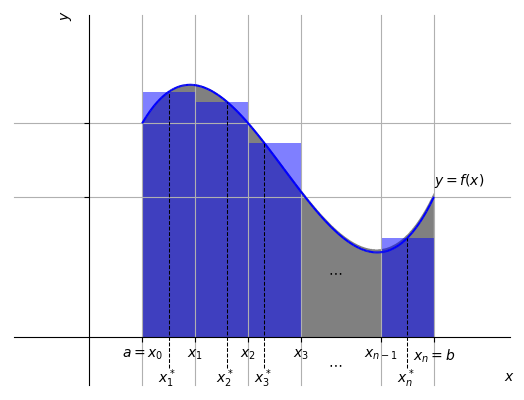
\includegraphics[width=0.9\textwidth]{figs/fig_soma_de_Riemann}
  \caption{Ilustração da soma de Riemann.}
  \label{fig:soma_de_Riemann}
\end{figure}

\begin{obs}\normalfont{(Aproximação da área sob o gráfico)}
No caso de uma função não negativa, uma soma de Riemann é uma aproximação da área sob seu gráfico e o eixo das abscissas\footnote{Veja o Exercício \ref{exer:int_geoRiemann} para uma interpretação geométrica no caso geral de funções contínuas.}. Veja a Figura \ref{fig:soma_de_Riemann}.
\end{obs}

\subsection{Integral definida}
A integral (definida) de $a$ até $b$ de uma dada função $f$ em relação a $x$ é denotada e definida por
\begin{equation}
  \int_a^b f(x)\,dx = \lim_{\|P\|\to 0} \sum_{i=1}^n f(x_i^*)\Delta x_i.
\end{equation}
De forma genérica, a integral definida de $a$ até $b$ é o limite das somas de Riemann quando a norma das partições $P$ do intervalo $[a, b]$ tendem a zero. Quando o limite existe, dizemos que $f$ é \textbf{integrável} no intervalo $[a, b]$.
\begin{figure}[H]
  \centering
  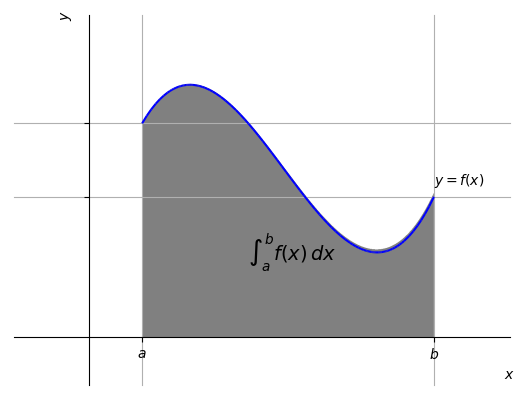
\includegraphics[width=0.75\textwidth]{figs/fig_geointdef}
  \caption{A integral definida como a área sob o gráfico.}
  \label{fig:geointdef}
\end{figure}
\nota{
Assim como foi estabelecido no caso da integral indefinida, temos na integral
\[ \mathlarger{\int}^{b}_{a}f(x)dx \]
\begin{enumerate}[a.]
    \item o símbolo \(\mathlarger{\int}\) é um \(S\) alongado que é chamado do símbolo de integração, e foi criado pelo matemático Leibniz para representar a palavra em latim \textbf{\textit{summa}};
    \item \(f(x)\) é o integrando;
    \item \(f(x)dx\) é o elemento de integração;
    \item \(a\) é o limite inferior e \(b\) é o limite superior;
    \item a variável de integração \(x\) não tem significado especial, pois
\[ \mathlarger{\int}^{b}_{a}f(x)dx= \mathlarger{\int}^{b}_{a}f(z)dz = \mathlarger{\int}^{b}_{a}f(t)dt = \mathlarger{\int}^{b}_{a}f(y)dy = \mathlarger{\int}^{b}_{a}f(u)du,\,\,\mbox{etc}. \]
\end{enumerate}
}\vspace{-0.5cm}
\nota{
Seja \(R\) a região região plana limitada pelo gráfico de \(f\), as retas \(x=a\), \(x=b\) e o eixo \(x\). 
\begin{itemize}
    \item Se \(f(x)\geq 0\), \(\forall\,x\in[a,b]\), então \(A_R=\mathlarger{\int}^{b}_{a}f(x)dx\) representa  a \textbf{área sob o gráfico}\footnote{Veja o Exercício \ref{exer:int_geointdef} para uma interpretação geométrica no caso geral de funções contínuas.} de $f$ que é delimitada pelo eixo $x$ e pelas retas $x=a$ e $x=b$. Veja a Figura \ref{fig:geointdef}.
    \item Se $f(x)\leq 0$ , \(\forall\,x\in[a,b]\), então \(-A_R=\mathlarger{\int}^{b}_{a}f(x)dx\) representa  a área delimitada pelo eixo $x$ e pelas retas $x=a$ e $x=b$
    
\end{itemize}
 \href{https://www.geogebra.org/m/ehzjmydv}{Neste endereço} há um Applet do GeoGebra com a ideia de integral como de retângulos formados sob uma curva.
}

\begin{ex}
  Vamos calcular
  \begin{equation*}
    \int_0^1 1\,dx
  \end{equation*}
  Aqui, o integrando é a função constante $f(x) = 1$ e o \emph{intervalo de integração} é $[0, 1]$. Sabemos que esta integral é a área sob o gráfico de $f$ no intervalo $[0, 1]$. Esta área é um retângulo de altura $1$ e comprimento $1$. Logo,
  \begin{equation*}
    \int_0^1 1\,dx = 1\cdot 1 = 1.
  \end{equation*}
\end{ex}

\subsection{Exercícios resolvidos}

\begin{exeresol}
  Calcule
  \begin{equation*}
    \int_{-1}^1 \sqrt{1 - x^2}\,dx
  \end{equation*}
\end{exeresol}
\begin{resol}
  Esta integral corresponde à área sob o gráfico da função $f(x) = \sqrt{1 - x^2}$ restrita ao intervalo $[-1, 1]$. Observando que
  \begin{align*}
    y = \sqrt{x^2 - 1} &\Rightarrow y^2 = 1 - x^2\\
                       &\Rightarrow y^2 + x^2 = 1,
  \end{align*}
  vemos que esta é a área do semicírculo de raio $1$. Logo,
  \begin{equation*}
    \int_{-1}^1 \sqrt{1 - x^2}\,dx = \frac{\pi \cdot 1^2}{2} = \frac{\pi}{2}
  \end{equation*}
\end{resol}

\begin{exeresol}
  Determine a função $F(x)$ tal que
  \begin{equation*}
    F(x) = \int_0^x t\,dt,
  \end{equation*}
  para todo $x\geq 0$. Então, mostre que $F'(x) = x$.
\end{exeresol}
\begin{resol}
  A integral definida
  \begin{equation*}
    \int_0^x t\,dt
  \end{equation*}
  é a área sob o gráfico de $f(t) = t$ restrita no intervalo $[0, x]$. Isto é, a área do triângulo retângulo de base $x$ e altura $x$. Logo,
  \begin{equation*}
    F(x) = \int_0^x t\,dt = \frac{x\cdot x}{2} = \frac{x^2}{2}
  \end{equation*}
  Ou seja, temos $F(x) = x^2/2$ e, portanto,
  \begin{equation*}
    F'(x) = \frac{1}{2}\cdot 2x = x.
  \end{equation*}
\end{resol}

\subsection{Exercícios}
\begin{multicols}{2}
\begin{exer}
  Calcule
  \begin{equation*}
    \int_{-1}^2 2\,dx
  \end{equation*}
\end{exer}
\begin{resp}
  $6$
\end{resp}

\begin{exer}
  Calcule
  \begin{equation*}
    \int_{-3}^{-1} 1-x\,dx
  \end{equation*}
\end{exer}
\begin{resp}
  $6$
\end{resp}


\begin{exer}
  Calcule
  \begin{equation*}
    \int_{-1}^2 -1\,dx
  \end{equation*}
\end{exer}
\begin{resp}
  $-3$
\end{resp}

\begin{exer}
  Calcule
  \begin{equation*}
    \int_{-1}^{1} x\,dx
  \end{equation*}
\end{exer}
\begin{resp}
  $0$
\end{resp}
\begin{exer}
  Determine $F(x)$ tal que
  \begin{equation*}
    F(x) = \int_{0}^{x} t+1\,dt.
  \end{equation*}
  para $x\geq 0$. Então, calcule $F'(x)$.
\end{exer}
\begin{resp}
  $\displaystyle F(x) = \frac{x^2}{2} + x$; $F'(x) = x + 1$.
\end{resp}
\end{multicols}
\begin{exer}\label{exer:int_geoRiemann}
  Faça uma interpretação geométrica da uma soma de Riemann aplicada a uma função contínua e não positiva. Estenda sua interpretação para funções contínuas arbitrárias.
\end{exer}
\begin{resp}
  Dica: a soma de Riemann é uma aproximação da área líquida sob o gráfico da função.
\end{resp}

\begin{exer}\label{exer:int_geointdef}
  Faça uma interpretação geométrica de
  \begin{equation*}
    \int_a^b f(x)\,dx
  \end{equation*}
  quando $f$ é uma função contínua e não positiva. Estenda sua interpretação para funções contínuas arbitrárias.
\end{exer}
\begin{resp}
  Dica: $\displaystyle \int_a^b f(x)\,dx$é a área líquida sob o gráfico da função.
\end{resp}



\section{Propriedades da integral definida}\hypertarget{PropIntDef}{}\label{sec:PropridIntDefinida}
Nesta seção apresentamos algumas propriedades da integral definida. Você verá que algumas já foram vistas na Seção \ref{sec:RegrasIntegracao} do capítulo anterior comuns a integral indefinida. 

Consideremos suas funções \(f\) e \(g\) integráveis em \([a,b]\) e \(k\) uma constante arbitrária em \(\mathbb{R}\), então:

\begin{enumerate}[1.]
\item $\displaystyle \int_a^a f(x)\,dx = 0$
\item $\displaystyle \int_a^b k\cdot f(x)\,dx = k\cdot\int_a^b f(x)\,dx$
\item $\displaystyle \int_a^b \left[f(x)\pm g(x)\right]\,dx = \int_a^b f(x)\,dx \pm \int_a^b g(x)\,dx$
\item $\displaystyle \int_a^b f(x)\,dx = \int_a^c f(x)\,dx + \int_c^b f(x)\,dx$
\item \( \mathlarger{\int}^{b}_{a}f(x)dx\, = - \mathlarger{\int}^{a}_{b}f(x)dx\)
\item  \(f(x)\geq 0\), \(\forall\,x\in[a,b]\), então \(\mathlarger{\int}^{b}_{a}f(x)dx\,\geq 0\);
\item Se \(f(x)\geq g(x)\), \(\forall\,x\in[a,b]\), então \(\mathlarger{\int}^{b}_{a}f(x)dx\,\geq \mathlarger{\int}^{b}_{a}g(x)dx\);
\item $\displaystyle \min_{x\in [a, b]} \{f(x)\}\cdot (b-a) \leq \int_a^b f(x)\,dx \leq \max_{x\in [a, b]} \{f(x)\}\cdot (b-a)$
\end{enumerate}

\begin{ex}
  Sejam $f$ e $g$ funções integráveis tais que
  \begin{align*}
    \int_{-1}^4 f(x)\,dx = 2,\\
    \int_4^5 f(x)\,dx = 3,\\
    \int_{-1}^4 g(x)\,dx = -1.
  \end{align*}
  Então, vejamos os seguintes casos:
  \begin{enumerate}[a)]
  \item
    \begin{equation*}
      \int_{4}^{-1} g(x)\,dx = -\int_{-1}^4 g(x)\,dx = -(-1) = 1.
    \end{equation*}
  \item
    \begin{equation*}
      \int_{-1}^{-1} 4f(x)\,dx = 0.
    \end{equation*}
  \item
    \begin{equation*}
      \int_{-1}^{4} -2g(x)\,dx = -2\int_{-1}^4 g(x)\,dx = 2.
    \end{equation*}
  \item
    \begin{align*}
      \int_{-1}^{4} \left[f(x) - 2g(x)\right]\,dx &= \int_{-1}^{4} f(x)\,dx - \int_{-1}^4 2g(x)\,dx \\
                                                  &= 2 - 2\int_{-1}^4 g(x)\,dx \\
                                                  &= 2 + 2 = 4.
    \end{align*}
  \item
    \begin{align*}
      \int_{-1}^5 f(x)\,dx &= \int_{-1}^4 f(x)\,dx + \int_{4}^5 f(x)\,dx \\
                           &= 2 + 3 = 5.
    \end{align*}
  \end{enumerate}
\end{ex}

\begin{ex}
  Lembrando que $-1 \leq \sen x \leq 1$, temos da propriedade e) acima que
  \begin{align}
    &2\pi \min_{x\in [-\pi, \pi]} \{\sen(x)\} \leq \int_{-\pi}^\pi \sen(x)\,dx \leq 2\pi \max_{x\in [\-pi, \pi]} \{\sen(x)\} \\
    &\Rightarrow -2\pi \leq \int_{-\pi}^\pi \sen(x)\,dx \leq 2\pi.
  \end{align}
\end{ex}

\section{Teorema do valor médio para integrais}\hypertarget{TVI}{}
Com base na noção de integral, define-se a média de uma função $f$ no intervalo $[a, b]$ por
\begin{equation}
  \frac{1}{b-a}\int_a^b f(x)\,dx,
\end{equation}
no caso de $f$ ser integrável neste intervalo.

\begin{framed}
\begin{teo}[\normalfont{(Teorema do valor médio para integrais)}]~\label{teo:int_teomed}
\\  Se $f$ for contínua em $[a, b]$, então existe $c\in [a, b]$ tal que
  \begin{equation}
    f(c) = \frac{1}{b-a}\int_a^b f(x)\,dx
  \end{equation}
  ou equivalentemente
  \begin{equation}
       \int_a^b f(x)\,dx=f(c) (b-a)
  \end{equation}
\end{teo}
\begin{framed}
\begin{dem}~
 \\ Vejamos uma ideia da demonstração. Da propriedade de integração e) acima, temos
  \begin{equation*}
    \min_{x\in [a, b]} \{f(x)\} \leq \frac{1}{b-a}\int_a^b f(x)\,dx \leq \max_{x\in [a, b]} \{f(x)\}
  \end{equation*}
  Agora, pelo Teorema do valor intermediário (Teorema \ref{teo:valorintermediario}), temos $f$ assume todos os valores entre seus valores mínimo e máximo. Logo, existe $c\in [a, b]$ tal que
  \begin{equation*}
    f(c) = \frac{1}{b-a}\int_a^b f(x)\,dx
  \end{equation*}  
\end{dem}\end{framed}\end{framed}
\nota{Como já foi dito, podemos interpretar a integral \(\mathlarger{\int}^{b}_{a}f(x)dx\) como a área da região limitada pelo gráfico de \(f\), pelas retas verticais \(x=a\) e \(x=b\) e pelo eixo \(x\), e mesmo assim, o Teorema 8.3 nos garante que existe um retângulo de largura \((b-a)\) e altura \(f(c)\) com a mesma área.}
\begin{ex}
  Seja $f$ uma função contínua em $[a, b]$, $a\neq b$, e
  \begin{equation*}
    \int_a^b f(x)\,dx = 0,
  \end{equation*}
  então $f$ possui pelo menos um zero neste intervalo. De fato, do Teorema do valor médio para integrais, temos que existe $c\in [a, b]$ tal que
  \begin{equation*}
    f(c) = \frac{1}{b-a}\int_a^b f(x)\,dx = \frac{1}{b-a}\cdot 0 = 0.
  \end{equation*}
\end{ex}

\section{Teorema Fundamental do Cálculo - parte I}\hypertarget{TFC}{}
Seja $f$ uma função integrável e $F$ a função definida por
\begin{equation}
  F(x) = \int_a^x f(t)\,dt,
\end{equation}
para algum número real $a$ dado.

\begin{framed}
\begin{teo}[Teorema Fundamental do Cálculo - TFC, parte I]~\label{teo:int_tfc1}
  Se $f$ é contínua em $[a, b]$, então é contínua em $[a, b]$ e diferenciável em $(a, b)$ a função
  \begin{equation}
    F(x) = \int_a^x f(t)\,dt
  \end{equation}
  sendo
  \begin{equation}
    F'(x) = \frac{d}{dx}\int_a^x f(t)\,dt = f(x).
  \end{equation}
\end{teo}
\begin{framed}
\begin{dem}~
 Vejamos a ideia da demonstração. Da definição de derivada, temos
  \begin{align*}
    F'(x) &= \lim_{h\to 0} \frac{F(x+h) - F(x)}{h} \\
          &= \lim_{h\to 0} \frac{1}{h}\left[\int_a^{x+h} f(x)\,dx - \int_a^x f(x)\, dx\right] \\
          &= \lim_{h\to 0} \frac{1}{h}\int_x^{x+h} f(x)\,dx
  \end{align*}
  Agora, do Teorema do valor médio para integrais (Teorema \ref{teo:int_teomed}), temos que existe $c_h \in [x, x+h]$ tal que
  \begin{equation*}
    f(c_h) = \frac{1}{x+h-x}\int_x^{x+h} f(x)\,dx = \frac{1}{h}\int_x^{x+h} f(x)\,dx
  \end{equation*}
  Notemos que $c_h\to x$ quando $h\to 0$ e, portanto, temos
  \begin{align*}
    F'(x) &= \lim_{h\to 0} \frac{1}{h}\int_x^{x+h} f(x)\,dx \\
          &= \lim_{h\to 0} f(c_h) \\
          &= f(x).
  \end{align*}
\end{dem}\end{framed}\end{framed}

\begin{ex}
  Vejamos os seguintes casos:
  \begin{multicols}{2}
  \begin{enumerate}[a)]
  \item
    $
      \frac{d}{dx}\int_1^x t^2\,dt = x^2.
    $
  \item
    $
      \frac{d}{dx}\int_0^x \sen(t)\,dt = \sen(x)
    $
  \end{enumerate}
  \end{multicols}
\end{ex}

A parte I do Teorema fundamental do cálculo (Teorema \ref{teo:int_tfc1}), mostra que a derivada da integral de uma função $f$ (contínua) é uma função $F$ tal que
\begin{equation}
  F'(x) = f(x).
\end{equation}
Como vimos no Capítulo anterior, $F$ é uma \emph{primitiva} da função $f$.

\section{Teorema fundamental do cálculo - parte II}
\begin{framed}\begin{teo}\normalfont{(Teorema fundamental do cálculo, parte II)}\label{teo:int_tfc2}
  Se $f$ é contínua em $[a, b]$ e $F$ é qualquer primitiva de $f$, então
  \begin{equation}
    \int_a^b f(x)\,dx = F(b) - F(a).
  \end{equation}
\end{teo}
\begin{framed}\begin{dem}
  Vejamos a ideia da demonstração. A parte I do Teorema fundamental do cálculo (Teorema \ref{teo:int_tfc1}), nos garante a existência de
  \begin{equation*}
    G(x) = \int_a^x f(t)\,dt.
  \end{equation*}
  Seja, então, $F$ uma primitiva qualquer de $f$. Logo,
  \begin{align*}
    F(b) - F(a) &= [G(b) + C] - [G(a) + C] \\
                &= G(b) - G(a) \\
                &= \int_a^b f(t)\,dx - \int_a^a f(t)\,dt \\
                &= \int_a^b f(t)\,dx
  \end{align*}
\end{dem}\end{framed}\end{framed}
\nota{Observemos que a diferença \(F(b)-F(a)\) é independente da eleição da antiderivada \(F\), pois todas as antiderivadas se diferenciam numa constante, que é eliminada ao ser efetuada a diferença. Por tal motivo, ao calcular uma integral definida não é necessário considerar a constante na antiderivada.}
\begin{ex}
  Vejamos os seguintes casos:
  \begin{enumerate}
  \item $\displaystyle \int_0^1 \,dx = \left. x \right|_0^1 = 1 - 0 = 1$
  \item $\displaystyle \int_0^1 x\,dx = \left.\frac{x^2}{2}\right|_0^1 = \frac{1^2}{2}-\frac{0^2}{2} = \frac{1}{2}$
  \item $\displaystyle \int_{-\frac{\pi}{2}}^{\frac{\pi}{2}} \cos(x)\,dx = \left.\sen(x)\right|_{-\frac{\pi}{2}}^{\frac{\pi}{2}} = \sen\left(\frac{\pi}{2}\right) - \sen\left(-\frac{\pi}{2}\right) = 2$
  \end{enumerate}
\end{ex}

\begin{obs}
  Do Teorema fundamental do cálculo, parte II, temos
  \begin{equation}
    \int_a^b f(x)\,dx = - \int_b^a f(x)\,dx
  \end{equation}
  De fato, se $F$ é uma primitiva de $f$, então
  \begin{align*}
    \int_a^b f(x)\,dx &= F(b) - F(a) \\
                      &= - \left[F(a) - F(b)\right] \\
                      &= - \int_b^a f(x)\,dx
  \end{align*}
\end{obs}

\begin{ex}
  Temos que
  \begin{equation*}
    \int_0^1 dx = \left. x\right|_0^1 = 1 - 0 = 1.
  \end{equation*}
  Agora,
  \begin{equation*}
    \int_1^0 dx = \left. x\right|_1^0 = 0 - 1 = -1.
  \end{equation*}
  Conforme esperado, temos
  \begin{equation*}
    \int_0^1 dx = - \int_1^0 dx
  \end{equation*}
\end{ex}
\begin{ex}
    \begin{align*}
    \int_{-1}^1 x^2\,dx &= \left.\frac{x^3}{3}\right|_{-1}^1 \\
                        &= \frac{1^3}{3} - \frac{(-1)^3}{3} \\
                        &= \frac{1}{3} + \frac{1}{3} = \frac{2}{3}
  \end{align*}
\end{ex}
\begin{ex}
  Vamos calcular
  \begin{equation*}
    \int_{0}^1 \pc{x^2 + 1}\,dx
  \end{equation*}
  Temos
  \begin{align*}
    \int \pc{x^2 + 1}\,dx &= \int x^2\,dx + \int \,dx\\
                     &= \frac{x^3}{3} + x + C
  \end{align*}
  Agora, do Teorema Fundamental do Cálculo, temos
  \begin{align*}
    \int_0^1 x^2+1\,dx &= \left. \frac{x^3}{3} + x\right|_0^1 \\
                       &= \frac{1}{3} + 1 - \left(\frac{0^3}{3} + 0\right) \\
                       &= \frac{4}{3}
  \end{align*}
\end{ex}
\subsection{Exercícios resolvidos}
\begin{exeresol}
Calculemos o valor numérico das seguintes integrais:
  \begin{compactenum}[a)]
  \item \( \mathlarger{\int}^{-1}_{1}\dfrac{1}{1+x^2}dx\)
  
  \begin{solution}
  Uma antiderivada de \(f(x)=\dfrac{1}{1+x^2}\) em \([-1,1]\) é \(F(x)={\rm arctg}(x)\), pela última nota, não é necessário considerar a constante de integração. Assim,

\[ \mathlarger{\int}^{-1}_{1}\dfrac{1}{1+x^2}dx = {\rm arctg}(x) \Big{|}^{1}_{-1} = {\rm arctg}( 1)- {\rm arctg}(-1) = \dfrac{\pi}{4}-\left(-\dfrac{\pi}{4} \right)=\dfrac{\pi}{2}. \]
  \end{solution}
  \item $\int_1^{\sqrt{e}} \pc{x - \frac{1}{x}}\,dx$
  
  \begin{resol}
  Primeiramente, notemos que
  \begin{align*}
    & \int x\,dx = \frac{x^2}{2} + C,\\
    & \int \frac{1}{x}\,dx = \ln x + C
  \end{align*}
  Então, usando as propriedades de integração, temos
  \begin{align*}
    \int_1^{\sqrt{e}} \pc{x - \frac{1}{x}}\,dx &= \int_1^{\sqrt{e}} x\,dx - \int_1^{\sqrt{e}} \frac{1}{x}\,dx \\
                                 &= \left[\frac{x^2}{2}\right]_1^{\sqrt{e}} - \left[\ln x\right]_1^{\sqrt{e}} \\
                                          &= \left[\frac{(\sqrt{e})^2}{2} - \frac{1}{2}\right] - \left[\ln\sqrt{e} - \ln 1\right]\\
                                          &= \frac{e}{2} - \frac{1}{2} - \frac{1}{2}\ln(e) - 0 \\
                                          &= \frac{e}{2} - 1.
  \end{align*}
\end{resol}

  \item \( \mathlarger{\int}^{\pi/2}_{0}{\rm sen\,}x\,dx\)\\
  
  \begin{solution}
  \[ \mathlarger{\int}^{\pi/2}_{0}{\rm sen\,}(x),dx \,= - \cos(x)\Big{|}^{\pi/2}_{0} = -\left(\cos\left(\dfrac{\pi}{2}\right) - \cos(0) \right)=1. \]
  \end{solution}
  \item \(\mathlarger{\int}^{1}_{0} e^x\,dx\)\\
  
  \begin{solution}
  \[ \mathlarger{\int}^{1}_{0} e^x\,dx\,= e^x \Big{|}^{1}_{0} = e^1-e^0=e-1. \]
  \end{solution}
  \item \( \mathlarger{\int}^{1}_{0} {\rm senh}( x)\,dx\)\\
  
  \begin{solution}
  \[ \mathlarger{\int}^{1}_{0} {\rm senh} (x)\,dx\,= \cosh(x) \Big{|}^{1}_{0} = \cosh(1) -1. \]
  \end{solution}
  \item \(\mathlarger{\int}^{1}_{-1}\dfrac{|x|}{1+x^2}dx\)\\
  
  \begin{solution}
  Da definição de \(f(x)=\dfrac{|x|}{1+x^2}\), temos que:

\[ f(x)=\left\{\begin{array}{ccl} \dfrac{x}{1+x^2},& & \mbox{se } x\geq 0;\\ \\ -\dfrac{x}{1+x^2},& & \mbox{se } x< 0. \end{array}\right. \]
Assim,

\[ \begin{array}{rcl} \mathlarger{\int}^{1}_{-1}f(x)dx &=& \mathlarger{\int}^{0}_{-1}f(x)dx + \mathlarger{\int}^{1}_{0}f(x)dx\\ &=& -\mathlarger{\int}^{0}_{-1}\dfrac{x}{1+x^2}dx + \mathlarger{\int}^{1}_{0}\dfrac{x}{1+x^2}dx\\ \\ &=& - \left[\dfrac{1}{2}\ln(1+x^2)\right]\Big{|}^{0}_{-1} + \left[\dfrac{1}{2}\ln(1+x^2)\right]\Big{|}^{1}_{0}\\ \\ &=& - \dfrac{1}{2}\left[\ln(1+0^2)-\ln(1+(-1)^2)\right] + \dfrac{1}{2}\left[\ln(1+1^2)- \ln(1+0^2)\right]\\ \\ &=& -\dfrac{1}{2}(-\ln 2) + \dfrac{1}{2}\ln 2 = \ln 2. \end{array} \]
  \end{solution}
  \item \(\mathlarger{\int}^{4}_{-4}|x^2+x-6|dx\)\\
  
  \begin{solution}
  Da definição de \(f(x)=|x^2+x-6|\), notamos que \(x^2+x-6=(x+3)(x-2)\), e assim, temos:

\[ f(x)\geq 0, \quad \mbox{se } x\in (-\infty,-3] \cup [2,+\infty) \quad \mbox{e}\quad f(x)\leq 0,\quad \mbox{se } x\in(-3,2). \] Logo, \[ f(x)= \left\{\begin{array}{ccl} x^2+x-6,& & \mbox{se } x\in (-\infty,-3] \cup [2,+\infty);\\ -(x^2+x-6),& & \mbox{se } x\in(-3,2). \end{array}\right. \]
Dessa forma, obtemos:

\[ \begin{array}{rcl} \mathlarger{\int}^{4}_{-4}|x^2+x-6|dx &=& \mathlarger{\int}^{-3}_{-4}(x^2+x-6)dx\,- \mathlarger{\int}^{2}_{-3}(x^2+x-6)dx\, + \mathlarger{\int}^{4}_{2}(x^2+x-6)dx\\ \\ &=& \left[\dfrac{x^3}{3}+ \dfrac{x^2}{2}-6x \right]\Big{|}^{-3}_{-4} - \left[\dfrac{x^3}{3}+ \dfrac{x^2}{2}-6x \right]\Big{|}^{2}_{-3} + \left[\dfrac{x^3}{3}+ \dfrac{x^2}{2}-6x \right]\Big{|}^{4}_{2}\\ \\ &=&\dfrac{17}{6} - \left(\dfrac{125}{6}\right) +\dfrac{38}{3}=\dfrac{109}{3}. \end{array} \]
  \end{solution}
  \end{compactenum}
\end{exeresol}




\begin{exeresol}
  Calcule a área entre o gráfico de $f(x) = \sen(x)$ e as retas $y=0$, $x=-\pi/2$ e $x=\pi/2$.
\end{exeresol}
\begin{resol}
  Lembrando que a integral definida está associada a área sob o gráfico do integrando, temos que a área desejada pode ser calculada por
  \begin{equation*}
    A = - \int_{-\frac{\pi}{2}}^0 \sen(x)\,dx + \int_0^{\frac{\pi}{2}} \sen(x)\,dx,
  \end{equation*}
  pois $\sen(x) < 0$ para $x\in (-\pi/2, 0)$ e $\sen(x) > 0$ para $x\in (0, \pi/2)$.
  Também, observamos que
  \begin{equation*}
    \int \sen(x)\,dx = -\cos(x) + C
  \end{equation*}
  Logo, do Teorema fundamental do cálculo segue que
  \begin{align*}
    A &= - \int_{-\frac{\pi}{2}}^0 \sen(x)\,dx + \int_0^{\frac{\pi}{2}} \sen(x)\,dx \\
      &= -\left[-\cos(x)\right]_{-\frac{\pi}{2}}^0 + \left[-\cos(x)\right]_0^{\frac{\pi}{2}} \\
      &= -[-1 - 0] + [-0 - (-1)] = 2. 
  \end{align*}
\end{resol}

\begin{exeresol}
  Encontre a função $y = y(x)$ tal que
  \begin{align*}
    \frac{dy}{dx} = x &\quad   \textrm{e}\quad y(0) = 1
  \end{align*}
  \end{exeresol}
\begin{resol}
  Integrando ambos os lados da equação diferencial em relação a $x$, temos
  \begin{equation*}
    \int \frac{dy}{dx}\,dx = \int x\,dx \Rightarrow y = \frac{x^2}{2} + C \\
  \end{equation*}
  Agora, da condição $y(0) = 1$, segue
  \begin{align*}
    y(0) = 1 &\Rightarrow \frac{0^2}{2} + C = 1 \\
             &\Rightarrow C = 1.
  \end{align*}
  Concluímos que $y = x^2/2 + 1$.
\end{resol}
\begin{exeresol}
  Calcule a área total entre as curvas $y=x^2-1$, $y=0$, $x=0$ e $x=2$.
  
  \begin{resol}
  Tendo em vista que $x^2-1\leq 0$ para $x\in [0, 1]$ e $x^2-1\geq [0, 1]$, temos que a área $A$ pedida é igual a
  \begin{equation*}
    A = -\int_0^1 x^2 -1\,dx + \int_1^2 x^2-1\,dx
  \end{equation*}
  Agora, calculamos a seguinte integral indefinida
  \begin{align*}
    \int x^2 - 1\,dx &= \int x^2\,dx - \int\,dx \\
                     &= \frac{x^3}{3} - x + C
  \end{align*}
  Então, usando o Teorema Fundamental do Cálculo, obtemos
  \begin{align*}
    A &= -\left[\frac{x^3}{3}-x\right]_0^1 + \left[\frac{x^3}{3}-x\right]_1^2\\
      &= - \left[\frac{1}{3}-1\right] + \left[\frac{8}{3} - 2 - \frac{1}{3} + 1\right] \\
      &= \frac{2}{3} \frac{4}{3} = 2.
  \end{align*}

Podemos usar o \geogebra~para calcular a área, com os seguintes comandos: \verb|-integral(x**2-1,0,1)+integral(x**2-1,1,2)|
\end{resol}
\end{exeresol}
\subsection{Exercícios}

\begin{exer}
  Sejam $f$ e $g$ tais que
  \begin{align*}
    &\int_{-2}^{0} f(x)\,dx = -2,& \int_{-1}^{0} f(x)\,dx = \frac{1}{2} &\qquad  \textrm{ e }     & \int_{-2}^0 g(x)\,dx = 1.
  \end{align*}
  Calcule
  \begin{multicols}{2}
  \begin{enumerate}[a)]
  \item $\displaystyle \int_{-1}^{-1} f(x) - 51\cdot g(x)\,dx$
  \item $\displaystyle \int_{-2}^{0} 2g(x) - \frac{1}{2}f(x)\,dx$
  \item $\displaystyle \int_{-2}^{-1} f(x)\,dx$
  \end{enumerate}
  \end{multicols}
\end{exer}

\begin{resp}
  a)~$0$; b)~$3$; c)~$-5/2$
\end{resp}

\begin{exer}
  Calcule
   \begin{multicols}{3}
  \begin{enumerate}[a)]
  \item $\displaystyle\int_{-1}^2 2\,dx$
  \item $\displaystyle\int_{-3}^{-1} 1-x\,dx$
  \item $\displaystyle\int_{1}^{e} \frac{2}{x}\,dx$
  \end{enumerate}
  \end{multicols}
\end{exer}
\begin{resp}
  a)~$6$; b)~$6$; c)~$2$
\end{resp}

\begin{exer}
  Calcule a área entre o gráfico de $f(x) = x^2-1$ e as retas $y=0$, $x=0$ e $x=2$.
\end{exer}
\begin{resp}
  $4/3$
\end{resp}
\begin{exer}
  Calcule a área total entre as curvas $y=x^3$, $y=0$, $x=-1$ e $x=1$.
\end{exer}
\begin{resp}
  $1/2$
\end{resp}
\begin{exer}
  Encontre a função $y = y(x)$ tal que
  \begin{align*}
    \frac{dy}{dx} = \cos(x), & y(\pi) = 1
  \end{align*}
 \end{exer}
\begin{resp}
  $y = \sen(x) + 1$
\end{resp}

\section{Mudança de Variável numa Integral Definida}
A regra de substituição para integrais definidas é
\begin{equation}
  \boldsymbol{\int_a^b f(u(x))u'(x)\,dx = \int_{u(a)}^{u(b)} f(u)\,du}
\end{equation}

\begin{ex}
  Vamos calcular
  \begin{equation*}
    \int_0^1 e^{-2x}\,dx
  \end{equation*}
  Por substituição, escolhemos
  \begin{equation*}
    u = -2x \Rightarrow du = -2dx
  \end{equation*}
  Logo,
  \begin{align*}
    \int_0^1 e^{-2x}\,dx &= \int_{u(0)}^{u(1)} e^{u}\frac{du}{-2} \\
                         &= -\frac{1}{2}\int_{0}^{-2} e^udu \\
                         &= -\frac{1}{2}\left[e^u\right]_0^{-2} \\
                         &= -\frac{1}{2}\left(e^{-2} - e^0\right) \\
                         &= \frac{1}{2} - \frac{e^{-2}}{2}
  \end{align*}

  Alternativamente, podemos calcular a integral indefinida primeiramente e, então, usar o Teorema Fundamental do Cálculo com a primitiva obtida. Ou seja, temos
  \begin{align*}
    \int e^{-2x}\,dx &= \int e^u\frac{du}{-2} \\
                     &= -\frac{1}{2}\int e^u\,du \\
                     &= -\frac{1}{2}e^u + C \\
                     &= -\frac{1}{2}e^{-2x} + C
  \end{align*}
  Então, do Teorema Fundamental do Cálculo, temos
  \begin{align*}
    \int_0^1 e^{-2x}\,dx &= \left[-\frac{1}{2}e^{-2x}\right]_0^1 \\
                         &= -\frac{1}{2}e^{-2} + \frac{1}{2}e^{0} \\
                         &= \frac{1}{2} - \frac{e^{-2}}{2},
  \end{align*}
  como esperado.


No \geogebra, utilizamos o comando: \verb|integral(exp(-2*x),0,1)|.
\end{ex}

\subsection{Exercícios Resolvidos}

\begin{exeresol}
  Calcule \(\mathlarger{\int}^{3}_{2} \dfrac{x^2}{(1+x^3)^3}\,dx\)\\
  
  \begin{solution}
  Considerando \(u=1+x^3\), obtemos \(du=3x^2\). Segue que para $x=2\Rightarrow u=9$ e para $x=3\Rightarrow u=28$. Fazendo estas substituições temos:
  \begin{align*}
      \mathlarger{\int}^{3}_{2} \dfrac{x^2}{(1+x^3)^3}\,dx &= \mathlarger{\int}^{28}_{9} \dfrac{du}{u^3}= \dfrac{1}{3} \mathlarger{\int}^{28}_{9} u^{-3}dt\\
      &=\dfrac{1}{3}\left(-\dfrac{1}{2}t^{-2}\right)=-\dfrac{1}{6}\dfrac{1}{t^2}\Big{|}^{28}_{9} = \dfrac{703}{381024}.
  \end{align*}


  \end{solution}
  \end{exeresol}

\begin{exeresol}
  Calcule
  \begin{equation*}
    \int_0^1x\sqrt{1-x^2}\,dx
  \end{equation*}
  \begin{resol}
  Vejamos as seguintes formas de calcular esta integral definida.
  \begin{itemize}
  \item {\bf Solução 1}: aplicando a regra de substituição em integrais definidas.
    \begin{equation*}
      \int_a^bf(u(x))u'(x)\,dx = \int_{u(a)}^{u(b)} f(u)\,du.
    \end{equation*}
    Escolhendo, $u = 1-x^2$, temos $du = -2x\,dx$. Daí, segue
    \begin{align*}
      \int_0^1x\sqrt{1-x^2}\,dx &= \int_{u(0)}^{u(1)}x\sqrt{u}\,\frac{du}{-2x}\\
                                &= -\frac{1}{2}\int_{1}^0 u^{\frac{1}{2}}\,du\\
                                &= -\frac{1}{2}\left.\frac{u^{\frac{1}{2}+1}}{\frac{1}{2}+1}\right|_{u=1}^0\\
                                &= -\frac{1}{3}\left.\sqrt{u^3}\right|_{u=1}^0\\
                                &= \frac{1}{3}
    \end{align*}
  \item {\bf Solução 2}: calculando uma primitiva em função de $x$.
    Para obtermos uma primitiva em função de $x$, calculamos a integral indefinida
    \begin{equation*}
      \int x\sqrt{1-x^2}\,dx
    \end{equation*}
    Como anteriormente, usamos a regra de substituição. Escolhendo $u=1-x^2$, temos $du = -2x\,dx$ e, portanto
    \begin{align*}
      \int x\sqrt{1-x^2}\,dx &= \int x\sqrt{u}\,\frac{du}{-2x}\\
                             &= -\frac{1}{2}\int u^{\frac{1}{2}}\,du\\
                             &= -\frac{1}{2}\frac{u^{\frac{1}{2}+1}}{\frac{1}{2}+1}\\
                             &= -\frac{1}{3}\sqrt{u^3}\\
                             &= -\frac{1}{3}\sqrt{(1-x^2)^3} + C
    \end{align*}
    Então, do teorema fundamental do cálculo, temos
    \begin{equation*}
      \int_0^1 x\sqrt{1-x^2}\,dx = -\frac{1}{3}\left.\sqrt{(1-x^2)^3}\right|_{0}^1 = \frac{1}{3}
    \end{equation*}
  \end{itemize}

  
  Para computarmos esta integral definida, podemos usar o seguinte comando do \geogebra: \verb|intgral(x*sqrt(1-x**2),0,1)|
\end{resol}
\end{exeresol}
\begin{exeresol}
  Calcule a área total entre as curvas $y=(1-x)^3$, $y=0$, $x=0$ e $x=2$.
  \begin{resol}
  A função $f(x) = (1-x)^3$ é positiva em $(0, 1)$ e negativa em $(1, 2)$. Logo, a área é igual a
  \begin{equation*}
    A = \int_0^1 (1-x)^3\,dx - \int_1^2 (1-x)^3\,dx
  \end{equation*}
  Agora, calculamos
  \begin{equation*}
    \int (1-x)^3\,dx
  \end{equation*}
  Para tanto, fazemos a substituição
  \begin{equation*}
    u = 1-x \Rightarrow du = -dx
  \end{equation*}
  Logo,
  \begin{align*}
    \int (1-x)^3\,dx &= -\int u^3du \\
                     &= -\frac{u^4}{4} + C \\
                     &= -\frac{(1-x)^4}{4} + C
  \end{align*}
  Então, do Teorema Fundamental do Cálculo, temos
  \begin{align*}
    A &= \left[-\frac{(1-x)^4}{4}\right]_0^1 - \left[-\frac{(1-x)^4}{4}\right]_1^2 \\
      &= \frac{1}{4} + \frac{1}{4} \\
      &= \frac{1}{2}
  \end{align*}

  
  No \geogebra, temos: \verb|integral((1-x)**3,0,1)-integral((1-x)**3,1,2)|
\end{resol}
\end{exeresol}
\subsection{Exercícios}

\begin{exer}
  Calcule
  \begin{equation*}
    \int_0^e \frac{\ln(x^3)}{x}\,dx
  \end{equation*}
\end{exer}
\begin{resp}
  $\displaystyle \frac{3\ln^2(x)}{2} + C$
\end{resp}

\begin{exer}
  Calcule
  \begin{equation*}
    \int_0^2 \frac{7}{(x-1)^2}\,dx
  \end{equation*}
\end{exer}
\begin{resp}
  $\frac{7}{2}$
\end{resp}

\begin{exer}
  Calcule
  \begin{equation*}
    \int_0^{\ln 3} e^{2x}\,dx
  \end{equation*}
\end{exer}
\begin{resp}
  $4$
\end{resp}

\begin{exer}
  Calcule
  \begin{equation*}
    \int_0^{\sqrt{e-1}} \frac{x}{x^2+1}\,dx
  \end{equation*}
\end{exer}
\begin{resp}
  $\frac{1}{2}$
\end{resp}

\section{Integração por Partes numa Integral Definida}
A ideia de integração por partes já foi vista no capítulo anterior, a única diferença é que agora temos
que considerar os limites de integração e desconsiderar a constante de integração. Dessa forma temos
o seguinte resultado:
\begin{equation}
  \boldsymbol{\int_{a}^b u\,dv = \left. uv \right|_{a}^b - \int_{a}^b v\,du}
\end{equation}
\begin{ex}
  Vamos usar a fórmula de integração por partes para integrais definidas para calcular
  \begin{equation*}
      \int_{-1}^1 xe^x\,dx
  \end{equation*}
  Para tanto, escolhemos $u = x$ e $dv = e^x$, donde
  \begin{align*}
    & u = x \Rightarrow du = dx \\
    & dv = e^{x}\,dx \Rightarrow v = \int e^{x}\,dx = e^{x}
  \end{align*}
  Segue da fórmula de integração por partes para integrais definidas que
   \begin{align*}
    \int_{-1}^1 xe^x\,dx &= \int_{-1}^1 u dv\\
                         &= uv|_{-1}^1 - \int_{-1}^1 vdu\\
                         &= xe^x|_{-1}^1 - \int_{-1}^1 e^x\,dx\\
                         &= e+e^{-1}-[e^x]_{-1}^1\\
                         &= e+e^{-1}-(e-e^{-1})\\
                         &= 2e^{-1}
  \end{align*}
  
  Para computarmos esta integral definida, podemos usar o seguinte comando do \geogebra:
\verb|integral(x*exp(x),-1,1)|
\end{ex}
\begin{ex}
  Vamos calcular
  \begin{equation*}
    \int_0^2 xe^{-x}\,dx
  \end{equation*}
  Para aplicar integração por partes, escolhemos
  \begin{align*}
    & u = x \Rightarrow du = dx \\
    & dv = e^{-x}\,dx \Rightarrow v = \int e^{-x}\,dx = -e^{-x}
  \end{align*}
  Segue da fórmula de integração por partes para integrais definidas que
  \begin{align*}
    \int_0^2 xe^{-x}\,dx &= \left. -xe^{-x}\right|_0^2 + \int_0^2 e^{-x}\,dx \\
                         &= -2e^{-2} + \left[-e^{-x}\right]_0^2 \\
                         &= -3e^{-2} + 1.
  \end{align*}

    No \geogebra~ utilize o comando:    \verb|integral(x*exp(-x),0,2)|
    \end{ex}
\subsection{Exercícios Resolvidos}
\begin{exeresol}
  Calculemos o valor da integral definida \(\mathlarger{\int}^{3}_{1} x^2 \ln(x)\,dx \)

\begin{solution}
Se consideramos

\[ \begin{array}{rclcrcl} u &=& \ln (x)&\quad\Rightarrow\quad& du &=& \dfrac{dx}{x}\\ dv &=& x^2\,dx &\quad\Rightarrow\quad& v &=& \mathlarger{\int}x^{2} dx \,\, =\,\,\dfrac{x^3}{3} \end{array} \]
obtemos:

\[ \mathlarger{\int}x^2\ln(x)\,dx=\dfrac{x^3}{3}\ln(x)- \mathlarger{\int} \dfrac{x^3}{3} \dfrac{dx}{x} =\dfrac{x^3}{3}\ln(x)- \dfrac{1}{3}\mathlarger{\int} x^2 dx =\dfrac{x^3 \ln(x)}{3}- \dfrac{x^3}{9}+c. \]
Logo

\[ \begin{array}{rclcr} \mathlarger{\int}^{3}_{1}x^2\ln(x)\,dx&=&\left[\dfrac{x^3}{3}\ln(x)- \dfrac{x^3}{9}\right]\Big{|}^{3}_{1}\\ \\ &=&\left[\dfrac{3^3}{3}\ln(3)- \dfrac{3^3}{9}\right]- \left[\dfrac{1^3}{3}\ln(1)- \dfrac{1^3}{9}\right] \\\\ &=&9\ln(3)- 3- 0+ \dfrac{1}{9}= 9\ln(3)-\dfrac{26}{9}. \end{array} \]
\end{solution}


\end{exeresol}
\section{Integrais Impróprias}
Na definição da integral definida \(\mathlarger{\int}^{b}_{a} f(x)\,dx\), foram estabelecidas duas restrições:
\begin{enumerate}[i.]
    \item O intervalo \([a,b]\) é limitado;
    \item A função \(f\) é limitada em \([a,b]\).
\end{enumerate}

Agora, estendemos a definição de integral definida retirando alguma dessas restrições. As integrais que possuem essas características são chamadas de \textit{integrais impróprias}:
\begin{itemize}
    \item Integrais impróprias com limites infinitos.
\item Integrais impróprias com limites finitos e \(f\) com uma descontinuidade infinita em \([a,b]\).
\end{itemize}
\subsection{Integrais Impróprias com Limites Infinitos}\hypertarget{LimInf}{}
\begin{framed}
\begin{definition}
Seja \(f\) uma função contínua no intervalo:
\begin{enumerate}[i.]
    \item \([a,\infty)\). A integral imprópria de $f$, de $a$ até  \(\infty\), é denotada e definida como:
\[ \mathlarger{\int}^{+\infty}_{a} f(x)\,dx\,:=\,\lim_{t\to+\infty} \mathlarger{\int}^{t}_{a} f(x)\,dx; \]
\item \((-\infty,b]\). A integral imprópria de \(f\), de \(-\infty\) até \(b\), é denotada e definida como:
\[ \mathlarger{\int}^{b}_{-\infty} f(x)\,dx\,:=\,\lim_{t\to-\infty} \mathlarger{\int}^{b}_{t} f(x)\,dx. \]
\end{enumerate}
Diz-se que \(\mathlarger{\int}^{+\infty}_{a} f(x)\,dx\) ou \(\mathlarger{\int}^{b}_{-\infty} f(x)\,dx\) \textbf{converge} quando esse limite existe. Caso contrário, diz-se que \textbf{diverge}.
\end{definition}
\end{framed}

Nas seções anteriores, se \(f(x)\geq 0\), a integral definida \(\mathlarger{\int}^{t}_{a} f(x)\,dx\) representa a área da região plana limitada pelo gráfico de \(f\), o eixo \(x\) e as retas verticais \(x=a\) e \(x=t\). No caso da integral imprópria ser convergente, podemos interpretar que o valor da integral:
\begin{compactenum}[a)]
\item \(\mathlarger{\int}^{+\infty}_{a} f(x)\,dx\) representa a área da região plana infinita que se encontra à direita da reta \(x=a\) e está compreendida entre o gráfico de \(f\) e o eixo \(x\). A figura à esquerda ilustra essa integral.
\begin{figure}[!htb]
    \centering
    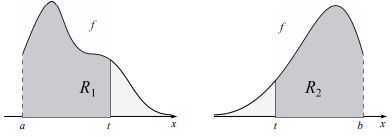
\includegraphics{figs/IntegralImpropria.png}
   % \caption{Caption}
    \label{fig:IntImpropria}
\end{figure}
\item \(\mathlarger{\int}^{b}_{-\infty} f(x)\,dx\) representa a área da região infinita que se encontra à esquerda da reta \(x=b\) e está compreendida entre o gráfico de \(f\) e o eixo \(x\). A figura à direita ilustra essa integral.
\end{compactenum}

\begin{framed}
\begin{definition}\label{def:IntImpInfinity}
Seja \(f\) uma função contínua e integrável no intervalo \((-\infty,\infty)\), então a integral imprópria de $f$, de $-\infty$ até \(\infty\), é denotada e definida como:

\[ \mathlarger{\int}^{+\infty}_{-\infty} f(x)\,dx\,:=\mathlarger{\int}^{c}_{-\infty} f(x)\,dx\,+ \mathlarger{\int}^{+\infty}_{c} f(x)\,dx, \]
onde \(c\) é um número real arbitrário.

Diz-se que a integral imprópria \(\mathlarger{\int}^{\infty}_{-\infty} f(x)\,dx\) \textbf{converge} quando $\mathlarger{\int}^{c}_{-\infty} f(x)\,dx$ e \(\mathlarger{\int}^{\infty}_{c} f(x)\,dx\) são convergentes, e \textbf{diverge} se alguma dessas integrais impróprias forem divergentes.
\end{definition}
\end{framed}

Na figura a seguir observamos 3 regiões: \(R_1\), \(R_2\) e \(R_3\):
\begin{figure}[H]
    \centering
    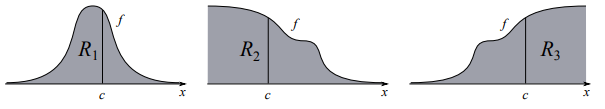
\includegraphics[width=\linewidth]{figs/IntImpropriaInfinity.png}
    %\caption{Caption}
    \label{fig:IntImpropriaInfinity}
\end{figure}
Logo, da Definição \ref{def:IntImpInfinity} podemos concluir que \(R_1\) gerará uma integral imprópria convergente, enquanto \(R_2\) e \(R_3\) gerarão integrais impróprias divergentes.
\begin{ex}
Determinemos se as seguintes integrais são convergentes ou divergentes:
\begin{enumerate}[a)]
\item \(\mathlarger{\int}^{2}_{-\infty} (x-2)e^x\,dx\)

\begin{solution}
Da definição da integral imprópria, obtemos que:

\[ \begin{array}{rcl} \mathlarger{\int}^{2}_{-\infty} (x-2)e^x\,dx &=& \lim\limits_{t\to -\infty}\mathlarger{\int}^{2}_{t} (x-2)e^x\,dx . \end{array} \] Aplicando integração por partes para $u=x-2$ e $dv=e^x dx$, temos que: \[ \begin{array}{rcl} \mathlarger{\int}^{2}_{t} (x-2)e^x\,dx &=& \left( (x-2)e^x -e^x \right)\Big{|}^{2}_{t}= (x-3)e^x\Big{|}^{2}_{t} \\ &=& (2-3)e^2 - (t-3)e^t = -e^2 - (t-3)e^t . \end{array} \] Assim, \[ \begin{array}{rcl} \mathlarger{\int}^{2}_{-\infty} (x-2)e^x\,dx &=& \lim\limits_{t\to -\infty} \left(-e^2 + (3-t)e^t \right) \,=\, -e^2 - \lim\limits_{t\to -\infty} (t-3)e^t . \end{array} \] Note que $t \to -\infty$ implica que $3-t \to + \infty\,$ e $\,e^t \to 0$. Logo, este último limite é da forma ``$\infty\cdot 0$''. Aplicando a *regra de L'Hôpital*, obtemos: \[ \lim\limits_{t\to -\infty} (t-3)e^t = \lim\limits_{t\to -\infty} \dfrac{t-3}{e^{-t}} = \lim\limits_{t\to -\infty} \dfrac{1}{-e^{-t}}=0. \]
Portanto,

\[ \mathlarger{\int}^{2}_{-\infty} (x-2)e^x\,dx=-e^2, \]
e concluímos que essa integral imprópria é convergente e converge a \(-e^2\).
\end{solution}
\item \(\mathlarger{\int}^{+\infty}_{1} \dfrac{x^2+2x}{x^3+3x^2+5}\,dx\)

\begin{solution}
\[ \begin{array}{rcl} \mathlarger{\int}^{+\infty}_{1} \dfrac{x^2+2x}{x^3+3x^2+5}\,dx &=& \lim\limits_{t\to +\infty}\mathlarger{\int}^{t}_{1} \dfrac{x^2+2x}{x^3+3x^2+5}\,dx. \end{array} \] Fazendo $z=x^3+3x^2+5$ temos que $dz=3(x^2+2x)dx$, e $x=1$ implica que $z=9$, e $x=t$ implica que $z=t^3+3t^2+5$. Assim, podemos fazer uma mudança de variável, isto é, \[ \begin{array}{rcl} \mathlarger{\int}^{t}_{1} \dfrac{x^2+2x}{x^3+3x^2+5}\,dx &=& \mathlarger{\int}^{t^3+3t^2+5}_{9}\dfrac{1}{3z}\,dz=\dfrac{1}{3} \ln|z|\Big{|}^{t^3+3t^2+5}_{9}=\dfrac{1}{3}\left[\ln|t^3+3t^2+5|- \ln(9)\right]. \end{array} \] Assim, \[ \begin{array}{rcl} \lim\limits_{t\to +\infty}\mathlarger{\int}^{t}_{1} \dfrac{x^2+2x}{x^3+3x^2+5}\,dx=\dfrac{1}{3} \lim\limits_{t\to +\infty}\left[\ln|t^3+3t^2+5|- \ln(9)\right]=\dfrac{1}{3}(+\infty)\,=\,+\infty. \end{array} \]
Portanto, a integral imprópria é divergente.
\end{solution}
\item \(\mathlarger{\int}^{+\infty}_{-\infty} \dfrac{dx}{1+x^2}\).

\begin{solution}
Escolhendo \(c=0\), obtemos:

\[ \begin{array}{rcl} \mathlarger{\int}^{+\infty}_{-\infty} \dfrac{dx}{1+x^2} &=&\mathlarger{\int}^{0}_{-\infty} \dfrac{dx}{1+x^2}\,+\,\mathlarger{\int}^{+\infty}_{0} \dfrac{dx}{1+x^2} = \lim\limits_{t\to -\infty} \mathlarger{\int}^{0}_{t} \dfrac{dx}{1+x^2}\,+\,\lim\limits_{t\to +\infty} \mathlarger{\int}^{t}_{0} \dfrac{dx}{1+x^2}\\ \\ &=& \lim\limits_{t\to -\infty} \left( {\rm arctg}(x) \Big{|}^{0}_{t}\right) + \lim\limits_{t\to +\infty} \left( {\rm arctg}(x) \Big{|}^{t}_{0}\right)\\ \\ &=& \lim\limits_{t\to -\infty} \left( {\rm arctg}(0)- {\rm arctg}(t)\right) + \lim\limits_{t\to +\infty} \left( {\rm arctg}(t)- {\rm arctg}(0)\right)\\ \\ &=& \lim\limits_{t\to -\infty} {\rm arctg}(t) + \lim\limits_{t\to +\infty} {\rm arctg}(t)\, =\, -\left(-\dfrac{\pi}{2}\right) + \dfrac{\pi}{2}=\pi. \end{array} \]
Portanto, a integral imprópria \(\mathlarger{\int}^{+\infty}_{-\infty} \dfrac{dx}{1+x^2}\) é convergente e converge em \(\pi\).
\end{solution}
\end{enumerate}
\end{ex}
\subsection{Integrais Impróprias com Limites Finitos}\hypertarget{LimInf2}{}
\begin{framed}
\begin{definition}\label{def:IntImpLimFinitos}
Seja \(f\) uma função contínua no intervalo:
\begin{enumerate}[i.]
    \item \([a,b)\) com \(\lim\limits_{x\to b^{-}}f(x)=\infty\). A integral imprópria de \(f\), de \(a\) até \(b\), é definida por:

\[ \mathlarger{\int}^{b}_{a} f(x)\,dx\,=\,\lim\limits_{t\to b^{-}} \mathlarger{\int}^{t}_{a} f(x)\,dx. \]
\item \((a,b]\) com \(\lim\limits_{x\to a^{+}}f(x)=\infty\). A integral imprópria de \(f\), de \(a\) até \(b\), é definida por:

\[ \mathlarger{\int}^{b}_{a} f(x)\,dx\,=\,\lim\limits_{t\to a^{+}} \mathlarger{\int}^{b}_{t} f(x)\,dx. \]
\item \([a,b]\), exceto em algum ponto \(c\in (a,b)\) onde \(\lim\limits_{x\to c^{-}}f(x)=\infty\) ou \(\lim\limits_{x\to c^{+}}f(x)=\infty\). A integral imprópria de \(f\), de \(a\) até \(b\), é definida por:

\[ \mathlarger{\int}^{b}_{a} f(x)\,dx\,=\,\mathlarger{\int}^{c}_{a} f(x)\,dx\,+\, \mathlarger{\int}^{b}_{c} f(x)\,dx. \]
\end{enumerate}
Diz-se que \(\mathlarger{\int}^{b}_{a} f(x)\,dx\) converge se os limites existem e, \(\mathlarger{\int}^{c}_{a} f(x)\,dx\,\) e \(\,\mathlarger{\int}^{b}_{c} f(x)\,dx\) são convergentes, respectivamente, caso contrário, diz-se que é divergente.
\end{definition}
\end{framed}

\nota{\begin{compactenum}[a)]
\item A Definição \ref{def:IntImpLimFinitos} pode ser estendida para \(n\) pontos de descontinuidade. Em outras palavras, seja \(f\) uma função definida em \((a,b)\), onde \(a\) pode ser \(-\infty\) e \(b\) pode ser \(\infty\). Se em $(a,b)$ existe um número finito de pontos $c_1,\,c_2,\ldots,\,c_n$ tal que $f$ tem descontinuidade infinita em $c_i$, isto é, $\lim\limits_{x\to c_i^-}f(x)=\infty$ ou \(\lim\limits_{x\to c_i^+}f(x)=\infty\) para \(i=1,\,\ldots,\,n\), então a integral da função \(f\) em \((a,b)\) é definida por:

\[ \mathlarger{\int}^{b}_{a} f(x)\,dx\,:=\,\mathlarger{\int}^{c_1}_{a} f(x)\,dx\,+\,\mathlarger{\int}^{c_2}_{c_1} f(x)\,dx\,+\cdots +\mathlarger{\int}^{b}_{c_n} f(x)\,dx. \]

Diz-se que \(\mathlarger{\int}^{b}_{a} f(x)\,dx\) é convergente se todas as integrais impróprias da direita são convergentes. Caso contrário, diz-se que é divergente.
\item Se \(f(x)\geq 0\) e a integral imprópria \(\mathlarger{\int}^{b}_{a} f(x)\,dx\) é convergente, o valor da integral representa a área da região infinita limitada pelo gráfico de \(f\), pelo eixo \(x\) e pelas retas \(x=a\) e \(x=b\).
\end{compactenum}}%

\begin{ex}
Determinemos se as seguintes integrais existem:
\begin{compactenum}[a)]
\item \(\mathlarger{\int}^{2}_{1} \dfrac{dx}{\sqrt{x-1}}\)

\begin{solution}
A função \(f(x)= \dfrac{1}{\sqrt{x-1}}\) é contínua em \((1,2]\) e \(\lim\limits_{x\to 1^{}}f(x)=\infty\). Assim,

\[ \mathlarger{\int}^{2}_{1} \dfrac{dx}{\sqrt{x-1}} = \lim\limits_{t\to 1^{+}}\mathlarger{\int}^{2}_{t} \dfrac{dx}{\sqrt{x-1}} = \lim\limits_{t\to 1^{+}}\left( 2\sqrt{x-1} \Big{|}^{2}_{t}\right) = \lim\limits_{t\to 1^{+}}\left( 2 - 2\sqrt{t-1} \right)=2. \]
Portanto, a integral imprópria é convergente e converge a \(2\).

Observe na figura abaixo que apesar da função $f$ (gráfico em vermelho) não está definida para $x=1$, ou seja, \(\lim\limits_{x\to 1^{-}}f(x)=\infty\), a sua primitiva $F(x)=2\sqrt{x-1}$ está definida para $x=1$, o que justifica  a sua  convergência pela possibilidade de se aplicar ambos os extremos do intervalo dado.
\end{solution}
\begin{figure}[htb]
    \centering
    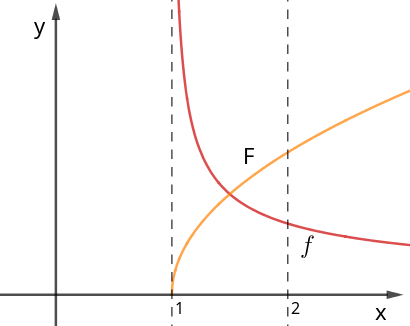
\includegraphics[scale=0.7]{figs/IntImpExConverge.png}
   % \caption{Caption}
    \label{fig:IntImpExConverge}
\end{figure}
\item \(\mathlarger{\int}^{\pi/4}_{-\pi/4} {\rm cotg} (\theta) \,d\theta\)

\begin{solution}
Ao definir a função \(f(\theta)={\rm cotg}(\theta) =\dfrac{\cos( \theta)}{{\rm sen}(\theta)}\), observamos que existe uma descontinuidade infinita em \(\theta=0\), isto é, \(\lim\limits_{\theta\to 0^{}}f(\theta)=\infty\) e \(\lim\limits_{\theta\to 0^{-}}f(\theta)=-\infty\). Assim,

\[ \mathlarger{\int}^{\pi/4}_{-\pi/4} {\rm cotg}(\theta) \,d\theta= \mathlarger{\int}^{0}_{-\pi/4} {\rm cotg}(\theta) \,d\theta\,+\,\mathlarger{\int}^{\pi/4}_{0} {\rm cotg}(\theta) \,d\theta \]
Por outro lado, a integral

\[ \begin{array}{rcl} \mathlarger{\int}^{0}_{-\pi/4} {\rm cotg}(\theta) \,d\theta&=&\lim\limits_{t \to 0^{-}} \mathlarger{\int}^{t}_{-\pi/4} {\rm cotg}(\theta) \,d\theta\,=\,\lim\limits_{t \to 0^{-}} \left(\ln |{\rm sen}(\theta) | \Big{|}^{t}_{-\pi/4}\right) \\ \\ &=&\lim\limits_{t \to 0^{-}} \left(\ln |{\rm sen}(t) | - \ln\left(\dfrac{\sqrt{2}}{2}\right) \right)=-\infty. \end{array} \]
Portanto, a integral imprópria é divergente.

Observe no gráfico da figura (a) abaixo que a primitiva  $F(x)=\frac{1}{2}\ln\left(-\cos^2 x+1\right)$ não está definida para $x=0$, o que justifica  a divergência de $\mathlarger{\int}^{0}_{-\pi/4} {\rm cotg}(\theta) \,d\theta$ e, consequentemente de $\mathlarger{\int}^{\pi/4}_{-\pi/4} {\rm cotg}(\theta) \,d\theta$, conforme comprovado nos cálculos.
\end{solution}
\begin{figure}[H]
    \centering
    \subfigure[]{\label{fig:intImpcot}%
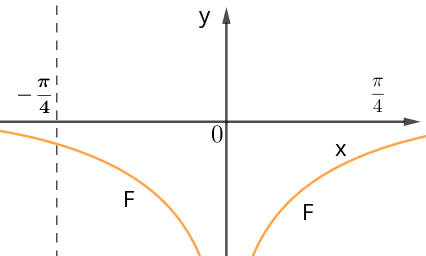
\includegraphics[width=0.45\textwidth]{figs/IntImpDivergenteEx1cot.png}}\quad
\subfigure[]{\label{fig:IntImpDiverg}%
 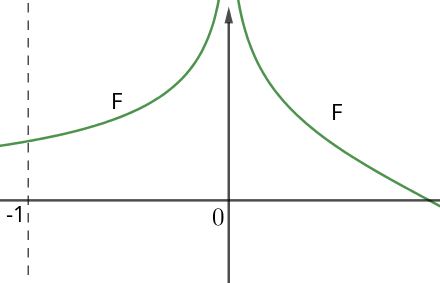
\includegraphics[width=0.45\textwidth]{figs/IntImpDivergenteEx2.png}}
\end{figure}
\item \(\mathlarger{\int}^{+\infty}_{-\infty} \dfrac{dx}{x(x-2)}\)

\begin{solution}
A função \(f(x)=\dfrac{1}{x(x-2)}\) tem duas descontinuidades infinitas em \(x=0\) e \(x=2\). Assim,

\[ \mathlarger{\int}^{+\infty}_{-\infty} \dfrac{dx}{x(x-2)}=\mathlarger{\int}^{0}_{-\infty} \dfrac{dx}{x(x-2)} + \mathlarger{\int}^{2}_{0} \dfrac{dx}{x(x-2)} + \mathlarger{\int}^{+\infty}_{2} \dfrac{dx}{x(x-2)}. \]
Já que essas integrais são impróprias em cada um dos extremos, precisamos trabalhar de forma análoga a da integral imprópria em \((-\infty, +\infty)\), ou seja, é necessário escolher 3 pontos, um em cada um desses intervalos. Escolhendo os pontos \(x=-1\in (-\infty, 0)\), \(x=1\in (0,2)\) e \(x=3\in (2, +\infty)\), a integral será expressada como:

\[ \begin{array}{rcl} \mathlarger{\int}^{+\infty}_{-\infty} \dfrac{dx}{x(x-2)}&=&\mathlarger{\int}^{-1}_{-\infty} \dfrac{dx}{x(x-2)} + \mathlarger{\int}^{0}_{-1} \dfrac{dx}{x(x-2)} + \mathlarger{\int}^{1}_{0} \dfrac{dx}{x(x-2)} \\ \\ && + \mathlarger{\int}^{2}_{1} \dfrac{dx}{x(x-2)} + \mathlarger{\int}^{3}_{2} \dfrac{dx}{x(x-2)} + \mathlarger{\int}^{+\infty}_{3} \dfrac{dx}{x(x-2)}. \end{array} \]

Agora, analisando a integral imprópria $\mathlarger{\int}^{0}_{-1} \dfrac{dx}{x(x-2)}$, temos que:
\[ \begin{array}{rcl} \mathlarger{\int}^{0}_{-1} \dfrac{dx}{x(x-2)}& =& \lim\limits_{t \to 0{-}}\mathlarger{\int}{t}_{-1} \dfrac{dx}{x(x-2)} = \lim\limits_{t \to 0^{-}} \left( \dfrac{1}{2} \ln \left|\dfrac{x-2}{x}\right| \Big{|}^{t}_{-1}\right) \\ \\ &=& \dfrac{1}{2}\lim\limits_{t \to 0^{-}} \left( \ln \left|\dfrac{t-2}{t} \right| - \ln (3) \right) \\ \\ &=& \dfrac{1}{2}\lim\limits_{t \to 0^{-}} \left( \ln \left|1- \dfrac{2}{t} \right| - \ln (3) \right) = +\infty. \end{array} \]

Portanto, a integral é divergente.

\nota{\textit{Observe no gráfico da figura (b) acima que a primitiva  $F(x)=-\frac{1}{2}\ln (|x|)+\frac{1}{2}\ln( |x-2|)$ não está definida para $x=0$, o que justifica  a divergência de $\mathlarger{\int}^{0}_{-1} \dfrac{dx}{x(x-2)}$ e, consequentemente de $\mathlarger{\int}^{-\infty}_{+\infty} \dfrac{dx}{x(x-2)}$, conforme comprovado nos cálculos.}}
\end{solution}
\end{compactenum}
\end{ex}
\section{Recapitulando}
Neste capítulo, apresentamos o conceito de integral definida, embora tenhamos usado as técnicas estudadas no capítulo anterior para resolvê-las, esse conceito é independente ao da integral indefinida e, por isso, foram tratados em capítulos diferentes.

Definimos a  integral de Riemann através de somatório. Em seguida, foram apresentadas as principais \hyperlink{PropIntDef}{propriedades da integral definida}. Entre os resultados mais importantes, apresentamos o \hyperlink{TVI}{teorema de valor intermediário} ou Teorema do valor médio para integrais e os \hyperlink{TFC}{teoremas fundamentais do cálculo integral}. E já que a teoria apresentada até aí resumia-se à função sobre um intervalo limitado, foi necessário estender a teoria de integral definida para \hyperlink{LimInf}{intervalos não limitados} e para funções com \hyperlink{LimInf2}{descontinuidade infinita}.









\end{document}